\label{appendix: code} 
 
All code is available at: \url{https://github.com/martkjoh/master}.


\section{Integrating the TOV equations}

For numerical integration of the TOV equations, we use SciPy's \texttt{integrate.solve\_ivp}.\footnote{
    Reference available here: \url{https://docs.scipy.org/doc/scipy/reference/generated/scipy.integrate.solve_ivp.html}.
    }
Equations of state are evaluated either as explicit functions if a closed-form is available or as an interpolating function is created using a cubic spline without smoothing.
All code is written using dimensionless variables, and setting $k_1 = k_2 = k_3$.
The TOV equation is then \autoref{TOV dimensionless}
%
\begin{align}
    \odv{\tilde m}{\tilde r} 
    = 3 \tilde r^2 \tilde u, \quad
    \odv{\tilde p}{\tilde r} 
     = - \frac{1}{\tilde r^2} \left(\tilde p + \tilde u\right) 
    \left(3  \tilde r^3 \tilde p + \tilde m\right) 
    \left(1 - \frac{2 \tilde m}{\tilde r}\right)^{-1}.
\end{align}
%
As $r \rightarrow 0$, parts of the TOV equation \autoref{TOV dimensionless} approaches a $0/0$-limit, and we must make use of an approximation for numeric evaluation.
The Taylor-expansion of the mass function around $\tilde r = 0$ is
%
\begin{equation}
    \tilde m(r) = \tilde m(0) + \tilde m'(0) \, \tilde r + \frac{1}{2!} \tilde m''(0) \tilde r^2
    + \frac{1}{3!} \tilde m'''(0) \tilde r^3 + \Oh\left(\tilde r^4\right).
\end{equation}
%
One of the boundary conditions is $\tilde m(0) = 0$.
We then use the differential equation for $\tilde m$, \autoref{diff eq mass}, to find
%
\begin{equation}
    \tilde m'(0) = 0, \quad
    \tilde m''(0) = 0, \quad
    \tilde m'''(0) = 6 k_2 \tilde u_0,
\end{equation}
%
where $\tilde u_0 = \tilde u(r = 0)$.
We get an approximation of the TOV equation for $\tilde r \ll 1$ by substituting the $\tilde m$ for its Taylor expansion and including only the leading-order term, which gives
%
\begin{equation}
    \odv{\tilde p}{\tilde r}
    \sim - \tilde r \, \left(\tilde p + \tilde u\right)
    \left( 3 \tilde p + \tilde u_0  \right)
    \left(1 - 2 \tilde u_0 \tilde r^2\right)^{-1}, \quad r\rightarrow 0
\end{equation}
%
For the Newtonian approximation to the TOV equation, we get
%
\begin{equation}
    \odv{\tilde p}{\tilde r} = -\frac{\tilde u \tilde m}{\tilde r^2}
    \sim - \tilde u \tilde u_0 \tilde r,  \quad r\rightarrow 0.
\end{equation}

 

\section{Spherically symmetric metric}
The calculations in \autoref{chapter: GR} were done using a CAS system.
The code is written in Python in a Jupyter notebook.
The full \texttt{.ipynb} file with executable code is available in the repository, at \url{https://github.com/martkjoh/master/blob/main/scripts/TOV.ipynb}
Below is some of the code, which illustrates the main functions and the outputs.

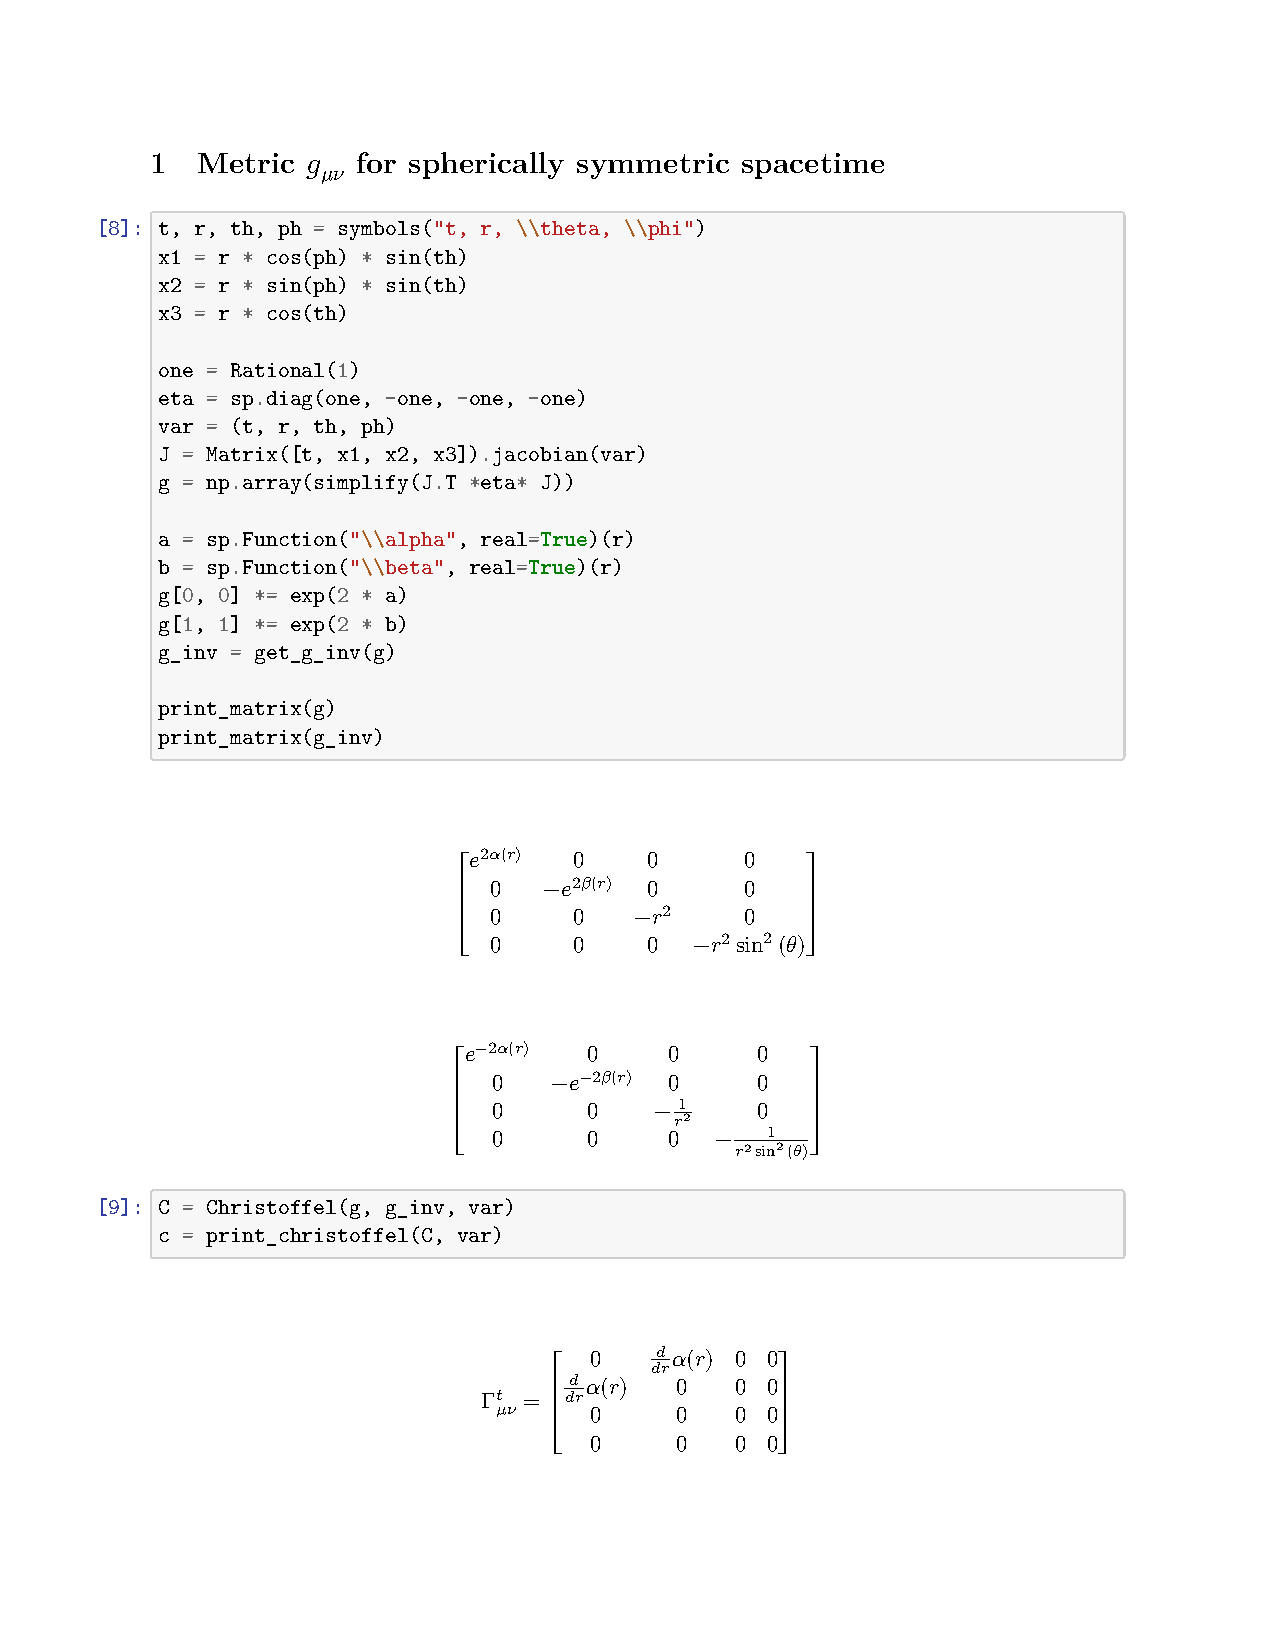
\includepdf[pages=-,pagecommand={},width=1.3\textwidth]{../scripts/TOV/TOV.pdf}

